
\section{Competition 1 Rules}

\paragraph{Overview}The first robot competition will be a race against the clock. Your robot will be timed as it follows a light masking tape path on a dark background. The team with the fastest cumulative time wins!
The "path following" competition will test your robot's navigation skills via light sensors. The key to a winning performance lies in your robot's light sensing and navigation algorithms.


The competition rules are as follows:
\begin{enumerate}
	\item The tape path will be continuous, i.e., no branches.
	\item The tape path will be between 0.5 and 1.5 inches wide.
	\item The tape path will not intersect itself.
	\item All tape path turns will be less than or equal to 135 degrees to the left or right of the robot's forward direction. For example, the tape path may take any angle inside the green circle below.
	\begin{figure}[h]
		\centering
		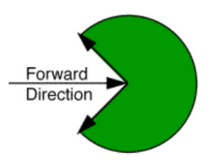
\includegraphics[width=0.2\linewidth]{figure01}
		\caption{}
		\label{fig:figure01}
	\end{figure}
	
	\item The shortest straight segment of the tape path will be 4 inches.
	\item The minimum distance from one segment of the tape to another, measured perpendicularly from the tape edge, will be 2 inches. In other words, you are guaranteed a 2 inch wide dark buffer on either side of the tape path, except when path angles are greater than 90 degrees. 
	\item The overall outside dimensions of the playing field will be 4 feet by 8 feet.
	\item Your robot will be positioned over the tape in whatever orientation you wish behind the starting line.
	\item The clock will stop when your robot's light sensors reach the end of the tape path.
	\item Each team will run two trials on its own individual chassis.
	\item The maximum time allowed per trial is 60 seconds. If your robot does not finish within 60 seconds, then its position will be recorded.
	\item If your robot leaves the tape path before the end, then its position will be recorded.
	\item If the centerpoint of your robot's body skips more than 4 inches of the tape path, then the robot will be stopped for "leaving the tape path".
	\item If no robot completes the path, then the robot which was closest to the finish during its trials will be declared the winner.
	\item You will be allowed to observe your robot's performance during both trials.
	\item You may modify your robot between trials.
	\item In each laboratory section, the top team will be awarded bonus points (0.2*teamwork\_score).
	\item The top four teams, across all of the laboratory sections, will compete in a lecture runoff on the Monday following the laboratory competitions.
	
\end{enumerate}
